\section{Extraction of Features}
This section discusses how the dataset has been gathered. Flurry Analytics is a powerful commercial tool that enables developers to analyze user's behavior in mobile applications through data observations.

Jungle Cubes and Dragon Cubes have an API installed that reports events to Flurry as long as the user is connected to the internet. Playing these games on offline mode will store such events on the local file of the device which will be sent to Flurry upon connecting to the internet.

The manner of reporting events is pretty straightforward. Figure \ref{fig:flurry_flow} shows the overview of the process of events reporting to Flurry. When an application starts, the timestamp and location (if possible to extract) is recorded and sends the data to Flurry. This means that the attribute, \textit{Session}, is incremented. If this is a first-time launch, then the \textit{Install Date} is reported to Flurry\footnote{Install Date information can be found in the application settings. If for example, user installed the app on date A, and decided to play it 5 days after, the value will always be date A (not A + 5)}. 
\begin{figure}[h]
\centering
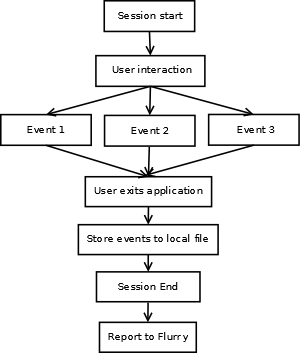
\includegraphics[scale=0.4]{figures/FlurryFlow.png} 
\caption{Overview of how events are recorded and reported to Flurry within an application's lifecycle}
\label{fig:flurry_flow}
\end{figure}

\subsection{Custom Events}
We define custom events significant for our analysis and adjust various game features as needed. These user interactions report different events which are triggered on specific parts of the game. For this paper, we only considered 3 custom events, \textit{LevelPlayedEvents, LevelSuccessEvents, LevelFailedEvents}. We will only consider these events and discuss points at which these events are triggered.

\begin{figure*}[h]
\centering

\includegraphics[scale=0.16]{figures/dnc_win.png} 
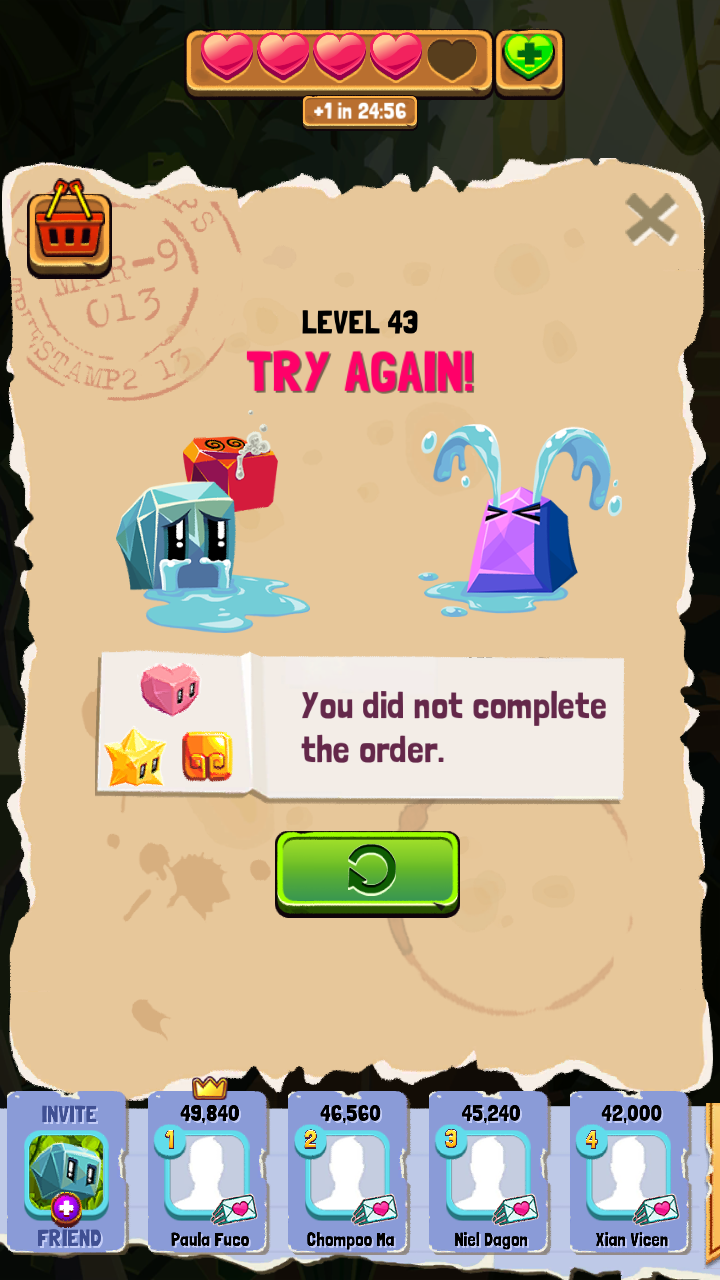
\includegraphics[scale=0.16]{figures/jnc_lose.png} 
\caption{Custom events defined in this paper are triggered when these screens are shown. DNC (left) shows a win result while JNC (right) shows a lose result.}
\label{fig:win_lose_sample}
\end{figure*}

Refer to Figure \ref{fig:win_lose_sample} as reference.\textit{LevelPlayedEvents} are triggered when the game results are shown to the user. This signifies that the game proper has concluded. In this figure, DNC and JNC will increment \textit{LevelPlayedEvents}.

\textit{LevelSuccessEvents} are triggered when the game results are shown and it has been concluded as a win result\footnote{A win for both games means that the objectives has been met by the user and can therefore proceed to the next level of the game. This is a positive event}. \textit{LevelFailedEvents} are triggered when the game results are shown as a fail result to the user\footnote{A fail for both games means that objectives were NOT met by the user. They have to repeat the level again. This is a negative event.}. In Figure \ref{fig:win_lose_sample}, the DNC shows a win result while JNC shows a fail result. DNC increments \textit{LevelSuccessEvents} while JNC increments \textit{LevelFailedEvents}.
